\chapter{INTRODUÇÃO}
A manufatura aditiva emerge como uma tecnologia altamente promissora para a produção de peças e componentes em diversas áreas, incluindo engenharia, medicina e a indústria aeroespacial. Suas características distintivas viabilizam a fabricação de peças complexas em pequenas quantidades, promovendo uma notável iterabilidade, bem como suportando a produção descentralizada. Nesse contexto, a impressão 3D, em particular o método de \textit{Fused Deposition Modeling} (FDM), ganha destaque crescente por se tornar cada vez mais acessível e disseminada.

A modelagem digital desempenha um papel essencial no processo de impressão 3D, trabalhando em conjunto com ferramentas como o \textit{Computer Aided Design} (CAD). Essa parceria possibilita a criação de modelos tridimensionais altamente precisos, que podem ser compartilhados e reproduzidos de forma descentralizada. Quando se trata de imprimir um desses modelos, existe uma série de etapas a serem realizadas, estas ilustradas no fluxograma da Figura \ref{fig:flowchart_intr}.

\begin{figure}[H]
    \begin{center}
        \caption{Fluxograma etapas Impressora 3D FDM}
        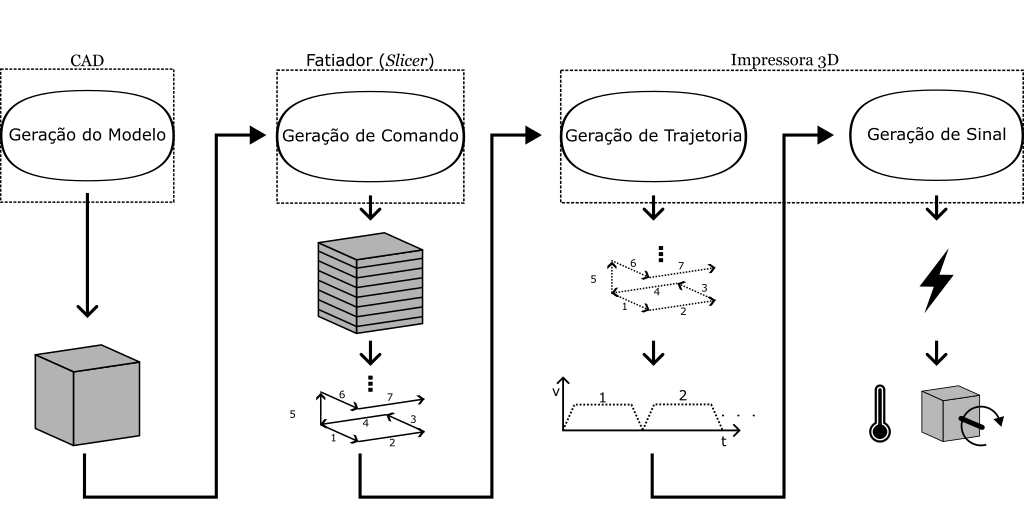
\includegraphics[scale=0.55]{flowchart_intr}

        \label{fig:flowchart_intr}
    \end{center}
\end{figure}

A primeira etapa prepara o modelo 3D o convertendo em uma série de comandos para a impressora, através de um software de fatiamento, conhecido como fatiador, ou do inglês \textit{slicer}. O \textit{slicer} divide o modelo em camadas e gera os comandos necessários para a impressora 3D, em geral esses comandos são representados pelo Gcode, uma linguagem de programação textual, nas impressoras FDM. Em sequência, a impressora, interpreta esses comandos para determinar como proceder e quando executar cada ação, por fim atuando os motores e outros dispositivos, como resistências elétricas para o aquecimento. É importante notar que entre a interpretação e a execução desses comandos existem diversos processos intermediários que exercem influência direta sobre a qualidade e a velocidade da impressão, sendo um deles a geração de trajetória, onde é construído o comportamento ao longo do tempo a ser executado pelos atuadores e dispositivos, por exemplo movimentos e mudanças de temperatura.

No entanto, uma das limitações significativas da impressão 3D, especialmente do tipo FDM, é o tempo de
impressão, que ainda restringe o tamanho das peças produzidas em um período razoável. Frequentemente, é
necessário utilizar camadas e linhas mais grossas para compensar esse aspecto, diminuindo a habilidade de
se reproduzir detalhes menores. Diante disso, existe uma procura por maneiras de se imprimir mais rapidamente,
sem comprometer a qualidade.

Assim, é relevante explorar técnicas que permitam alcançar capacidades superiores de qualidade e
velocidade de impressão, flexibilizando a tecnologia e ampliando sua aplicação comercial viável.

Este trabalho tem como objetivo geral investigar e desenvolver uma metodologia para atuação de controle na geração de
comandos em impressoras 3D utilizando o método FDM de forma a possibilitar maiores velocidades e garantindo a precisão dimensional das peças produzidas. E os seguintes objetivos específicos: 
\begin{itemize}
    \item Desenvolver um algoritmo iterativo que possa ser integrado ao sistema de controle de impressoras 3D para minimizar os desvios entre o percurso desejado e o efetivamente percorrido, levando em consideração a dinâmica da impressora.
    \item Simular o comportamento da impressora 3D com o novo algoritmo para avaliar o comportamento do método em relação aos parâmetros controlados.
\end{itemize}


